\documentclass[a4paper,12pt]{article}
\usepackage[T2A]{fontenc}
\usepackage[utf8]{inputenc}
\usepackage[russian]{babel}
\usepackage{graphicx} % Для вставки изображений
\usepackage{float}    % Для точного позиционирования
\usepackage{subcaption}
\usepackage{amsmath, amssymb}
\usepackage{geometry}
\geometry{top=2cm, bottom=2cm, left=3cm, right=1.5cm}

\begin{document}

\thispagestyle{empty}
\begin{center}
    \large
    Министерство науки и высшего образования Российской Федерации\\
    Федеральное государственное автономное образовательное учреждение\\
    высшего образования\\
    «Национальный исследовательский университет ИТМО»\\
    \vspace{5cm}
    \textbf{Отчёт по исследовательской работе № 1}\\
    \textbf{По предмету: Математический анализ и основы вычислений}\\
    \vspace{6cm}
    \begin{flushright}
        Выполнил работу:\\ Тиганов Вадим Игоревич\\
        \vspace{1cm}
        Академическая группа: \\ J3112\\
        \vspace{1cm}
        Вариант: \\18
    \end{flushright}
    \vspace{1cm}
    \vspace{3cm}
    \begin{center}
        Санкт-Петербург, 2025\\
    \end{center}
\end{center}

\newpage

\tableofcontents

\newpage

\section{Цель и задачи}
\textbf{Цель работы:} применить навыки, полученные за время второго семестра по предмету Математический анализ для решения практических задач вручную и с помощью программного обеспечения.\\
\textbf{Задачи работы:}
\begin{enumerate}
    \item Применить теоретические знания для оперирования интегральными суммами и для приведения выражений к таковым.
    \item Решить заданные практические задания вручную и проверить ответ.
    \item Визуализировать графики функций, где это требуется.
    \item Реализовать решение задачи на ЯП в последней части работы.
\end{enumerate}

\section{Ход работы}

\subsection{Задание 1}

Рассмотрим функцию
\[
f(x) = \frac{x^2 + 1}{x - 1}.
\]
Исследовать на равномерную непрерывность на множествах\\
\emph{(a)} \( X = [3, +\infty) \) \\
\emph{(b)} \( X = (1, 3) \)\\

\begin{figure}[h] % [h] - разместить "здесь" (here)
    \centering % Центрирование
    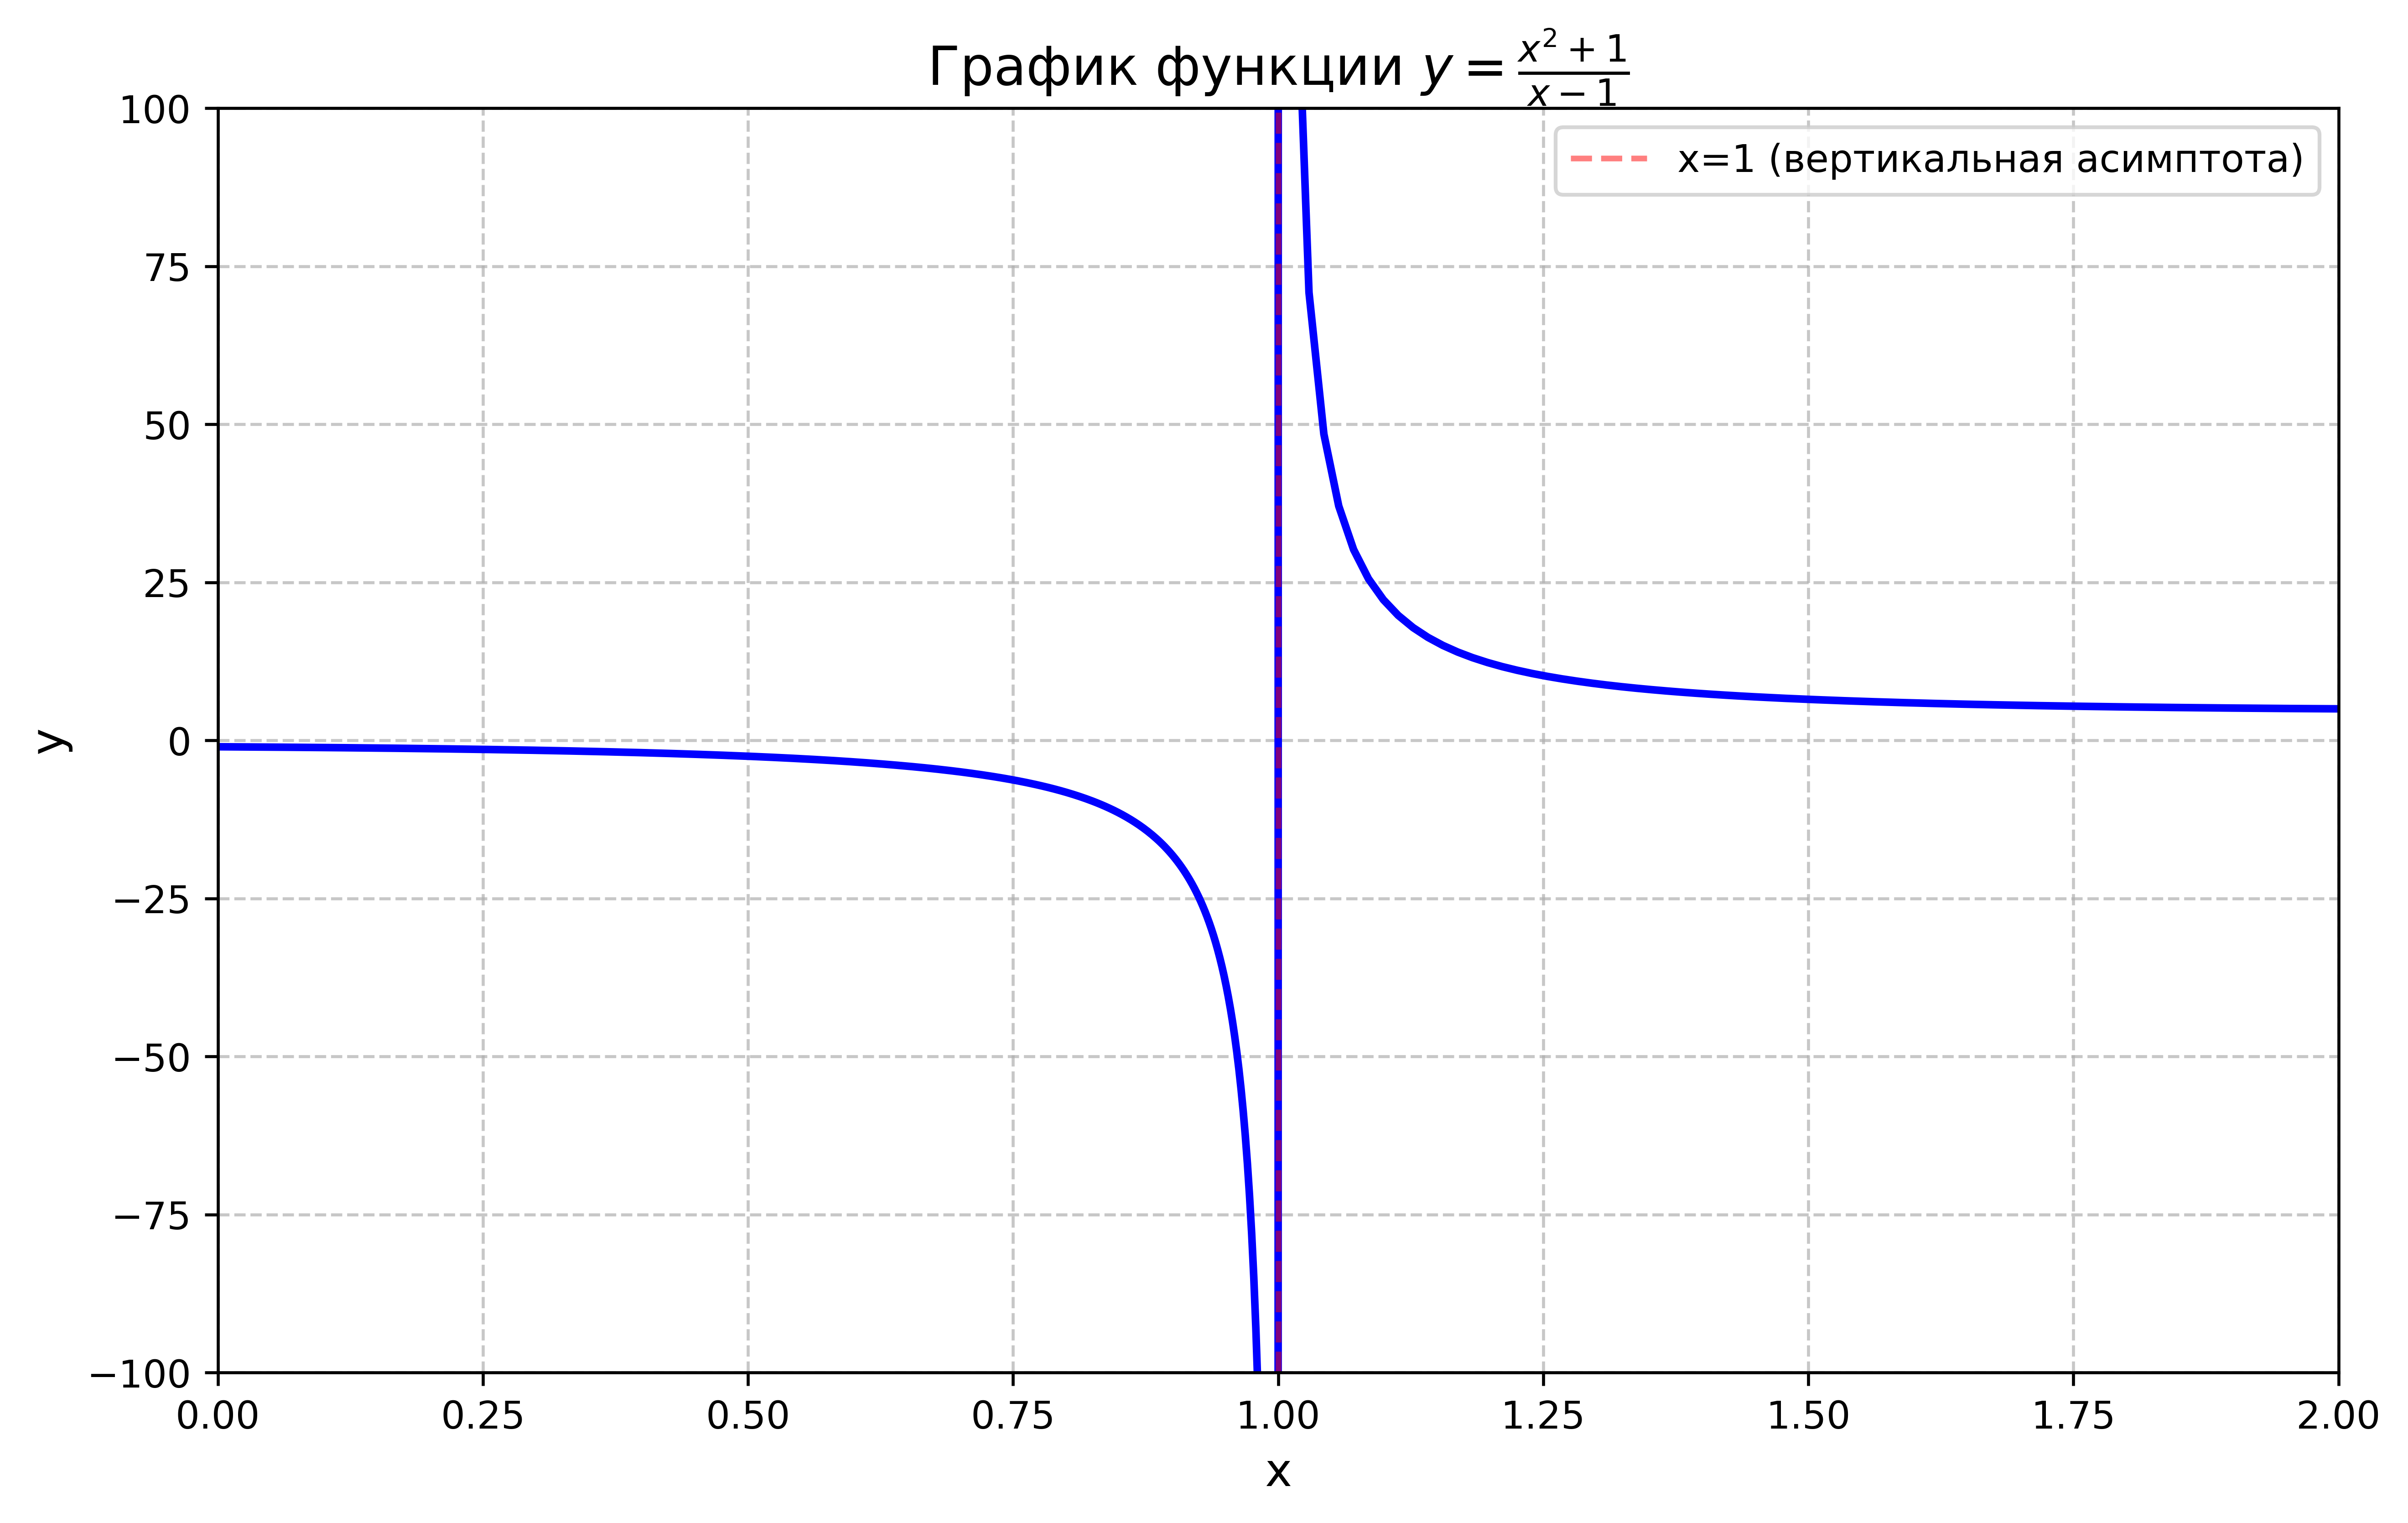
\includegraphics[width=0.8\textwidth]{img/task1_graph.png} % Ширина = 80% от ширины текста
    \caption{График функции \( f(x) = \frac{x^2 + 1}{x - 1} \)}
    \label{fig:graph}
\end{figure}
\emph{Решение задачи:}

\begin{figure}[H]
    \centering
    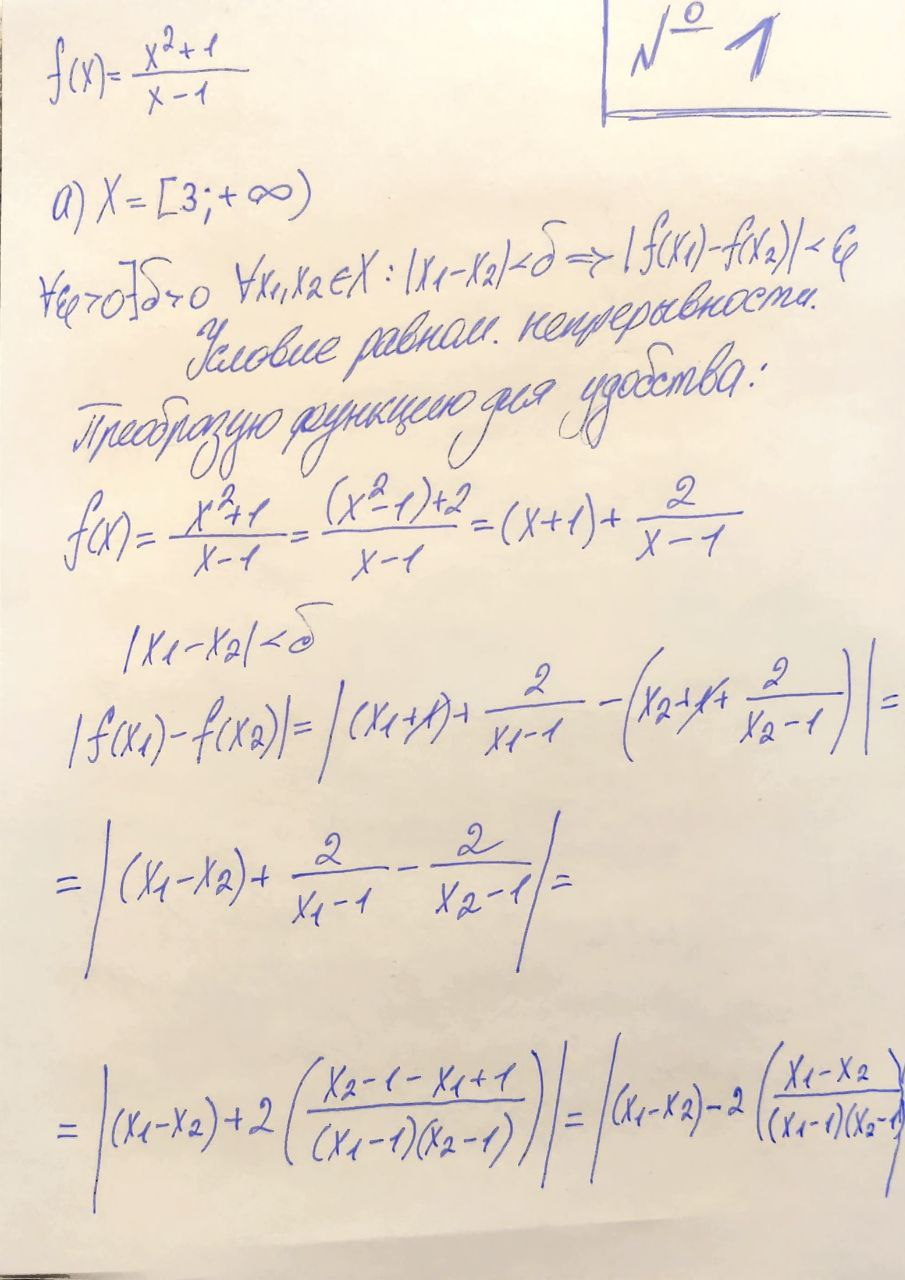
\includegraphics[width=0.8\linewidth]{img/1_1.jpg}
    \caption{\emph{(a)}}
    \label{fig:part1}
\end{figure}

\begin{figure}[H]
    \centering
    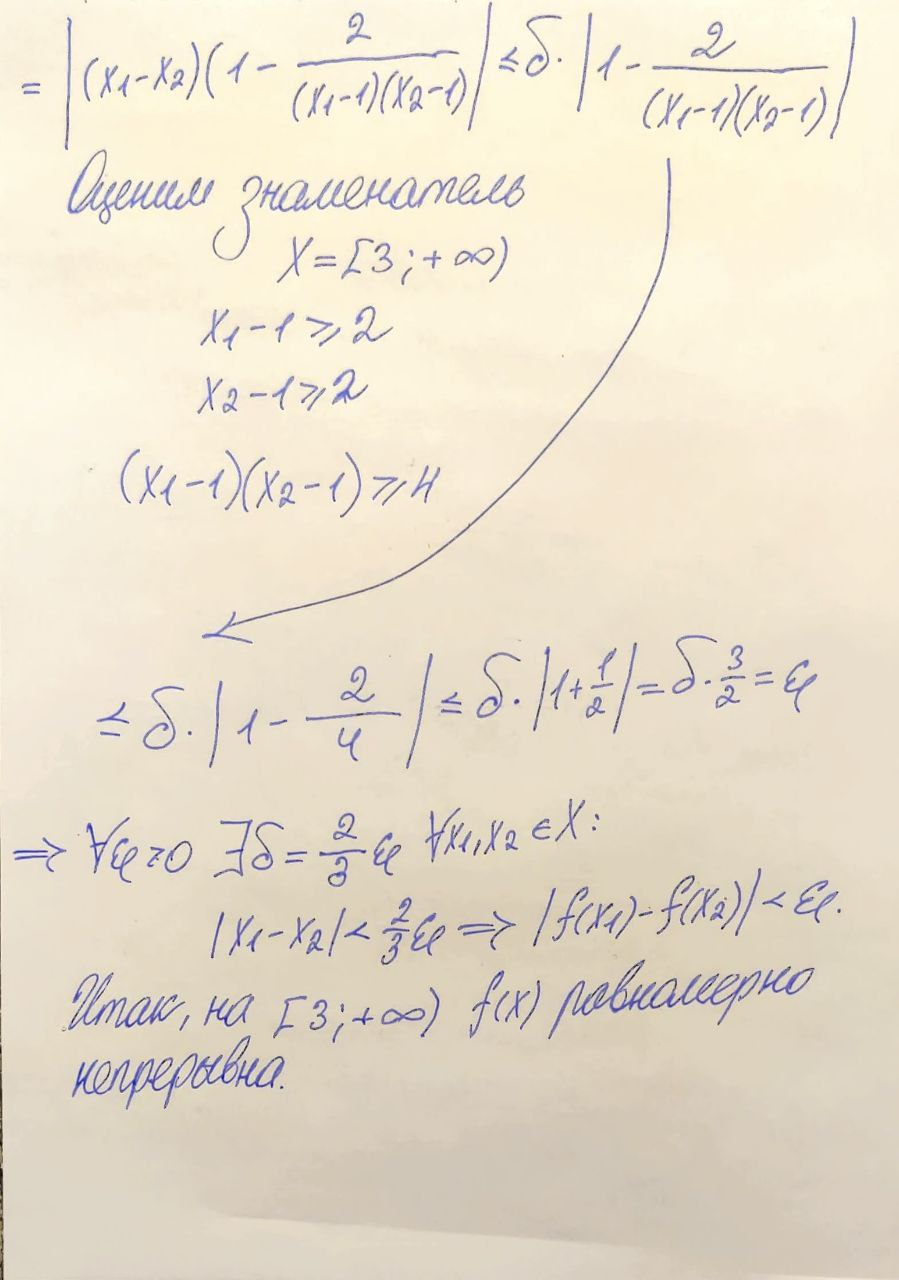
\includegraphics[width=0.8\linewidth]{img/1_2.jpg}
    \caption{\emph{(a)}}
    \label{fig:part2}
\end{figure}

\begin{figure}[H]
    \centering
    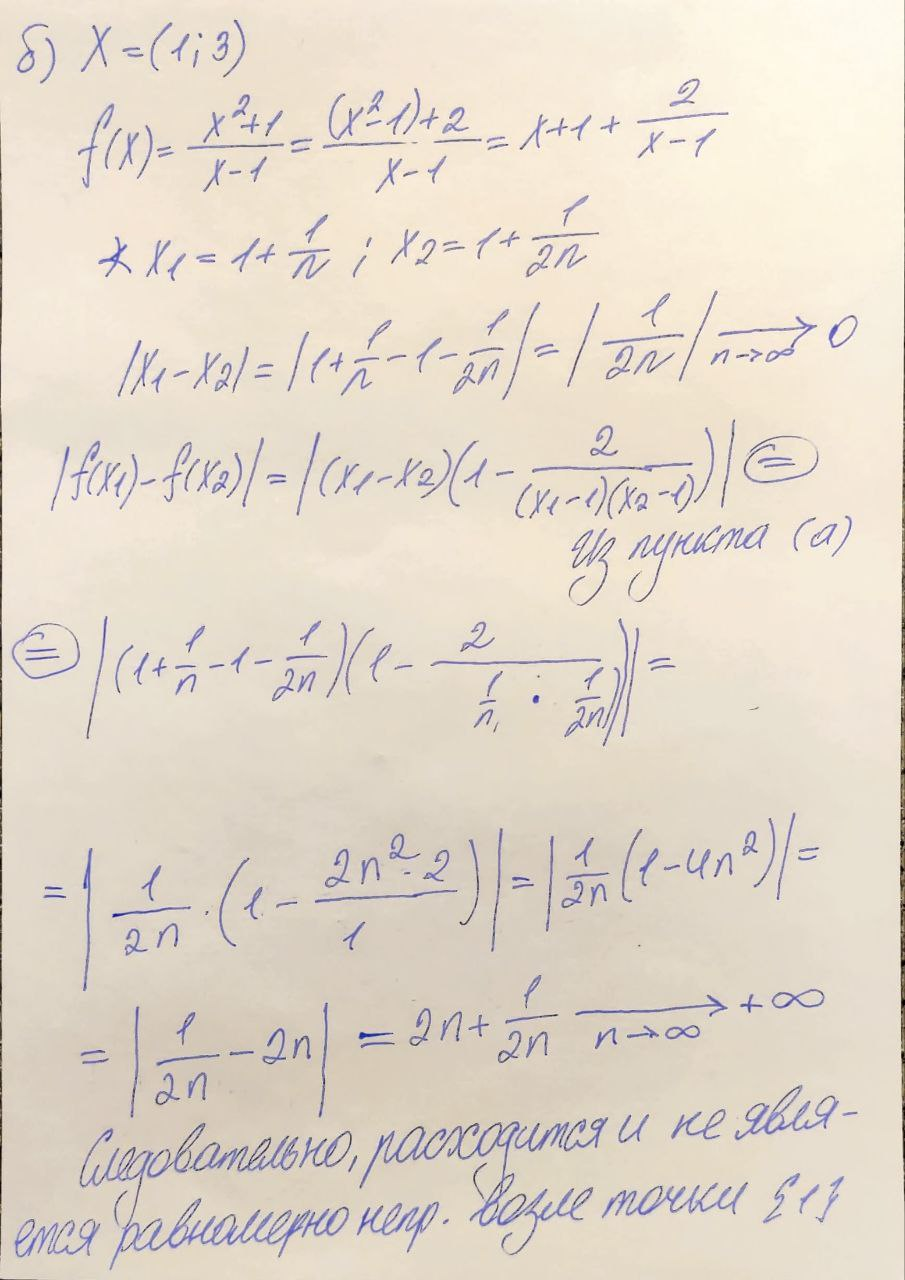
\includegraphics[width=0.8\linewidth]{img/1_3.jpg}
    \caption{\emph{(b)}}
    \label{fig:part3}
\end{figure}

Итак, задача решена. Функция \( f(x) \) является равномерно непрерывной на промежутке \(X = [3,+\infty)\), и не является таковой на промежутке \( X = (1,3) \)


\newpage
\subsection{Задание 2}

Требуется:
\begin{enumerate}
    \item Преобразовать выражение к интегральной сумме,
    \item Доказать существование соответствующего интеграла,
    \item Найти предел:
\end{enumerate}

\[
\lim_{n \to \infty} \sum_{k=1 - n}^{n} \frac{k}{kn + 2n^2}
\]

\subsection*{Графическая интерпретация интеграла}

\begin{figure}[H]
    \centering
    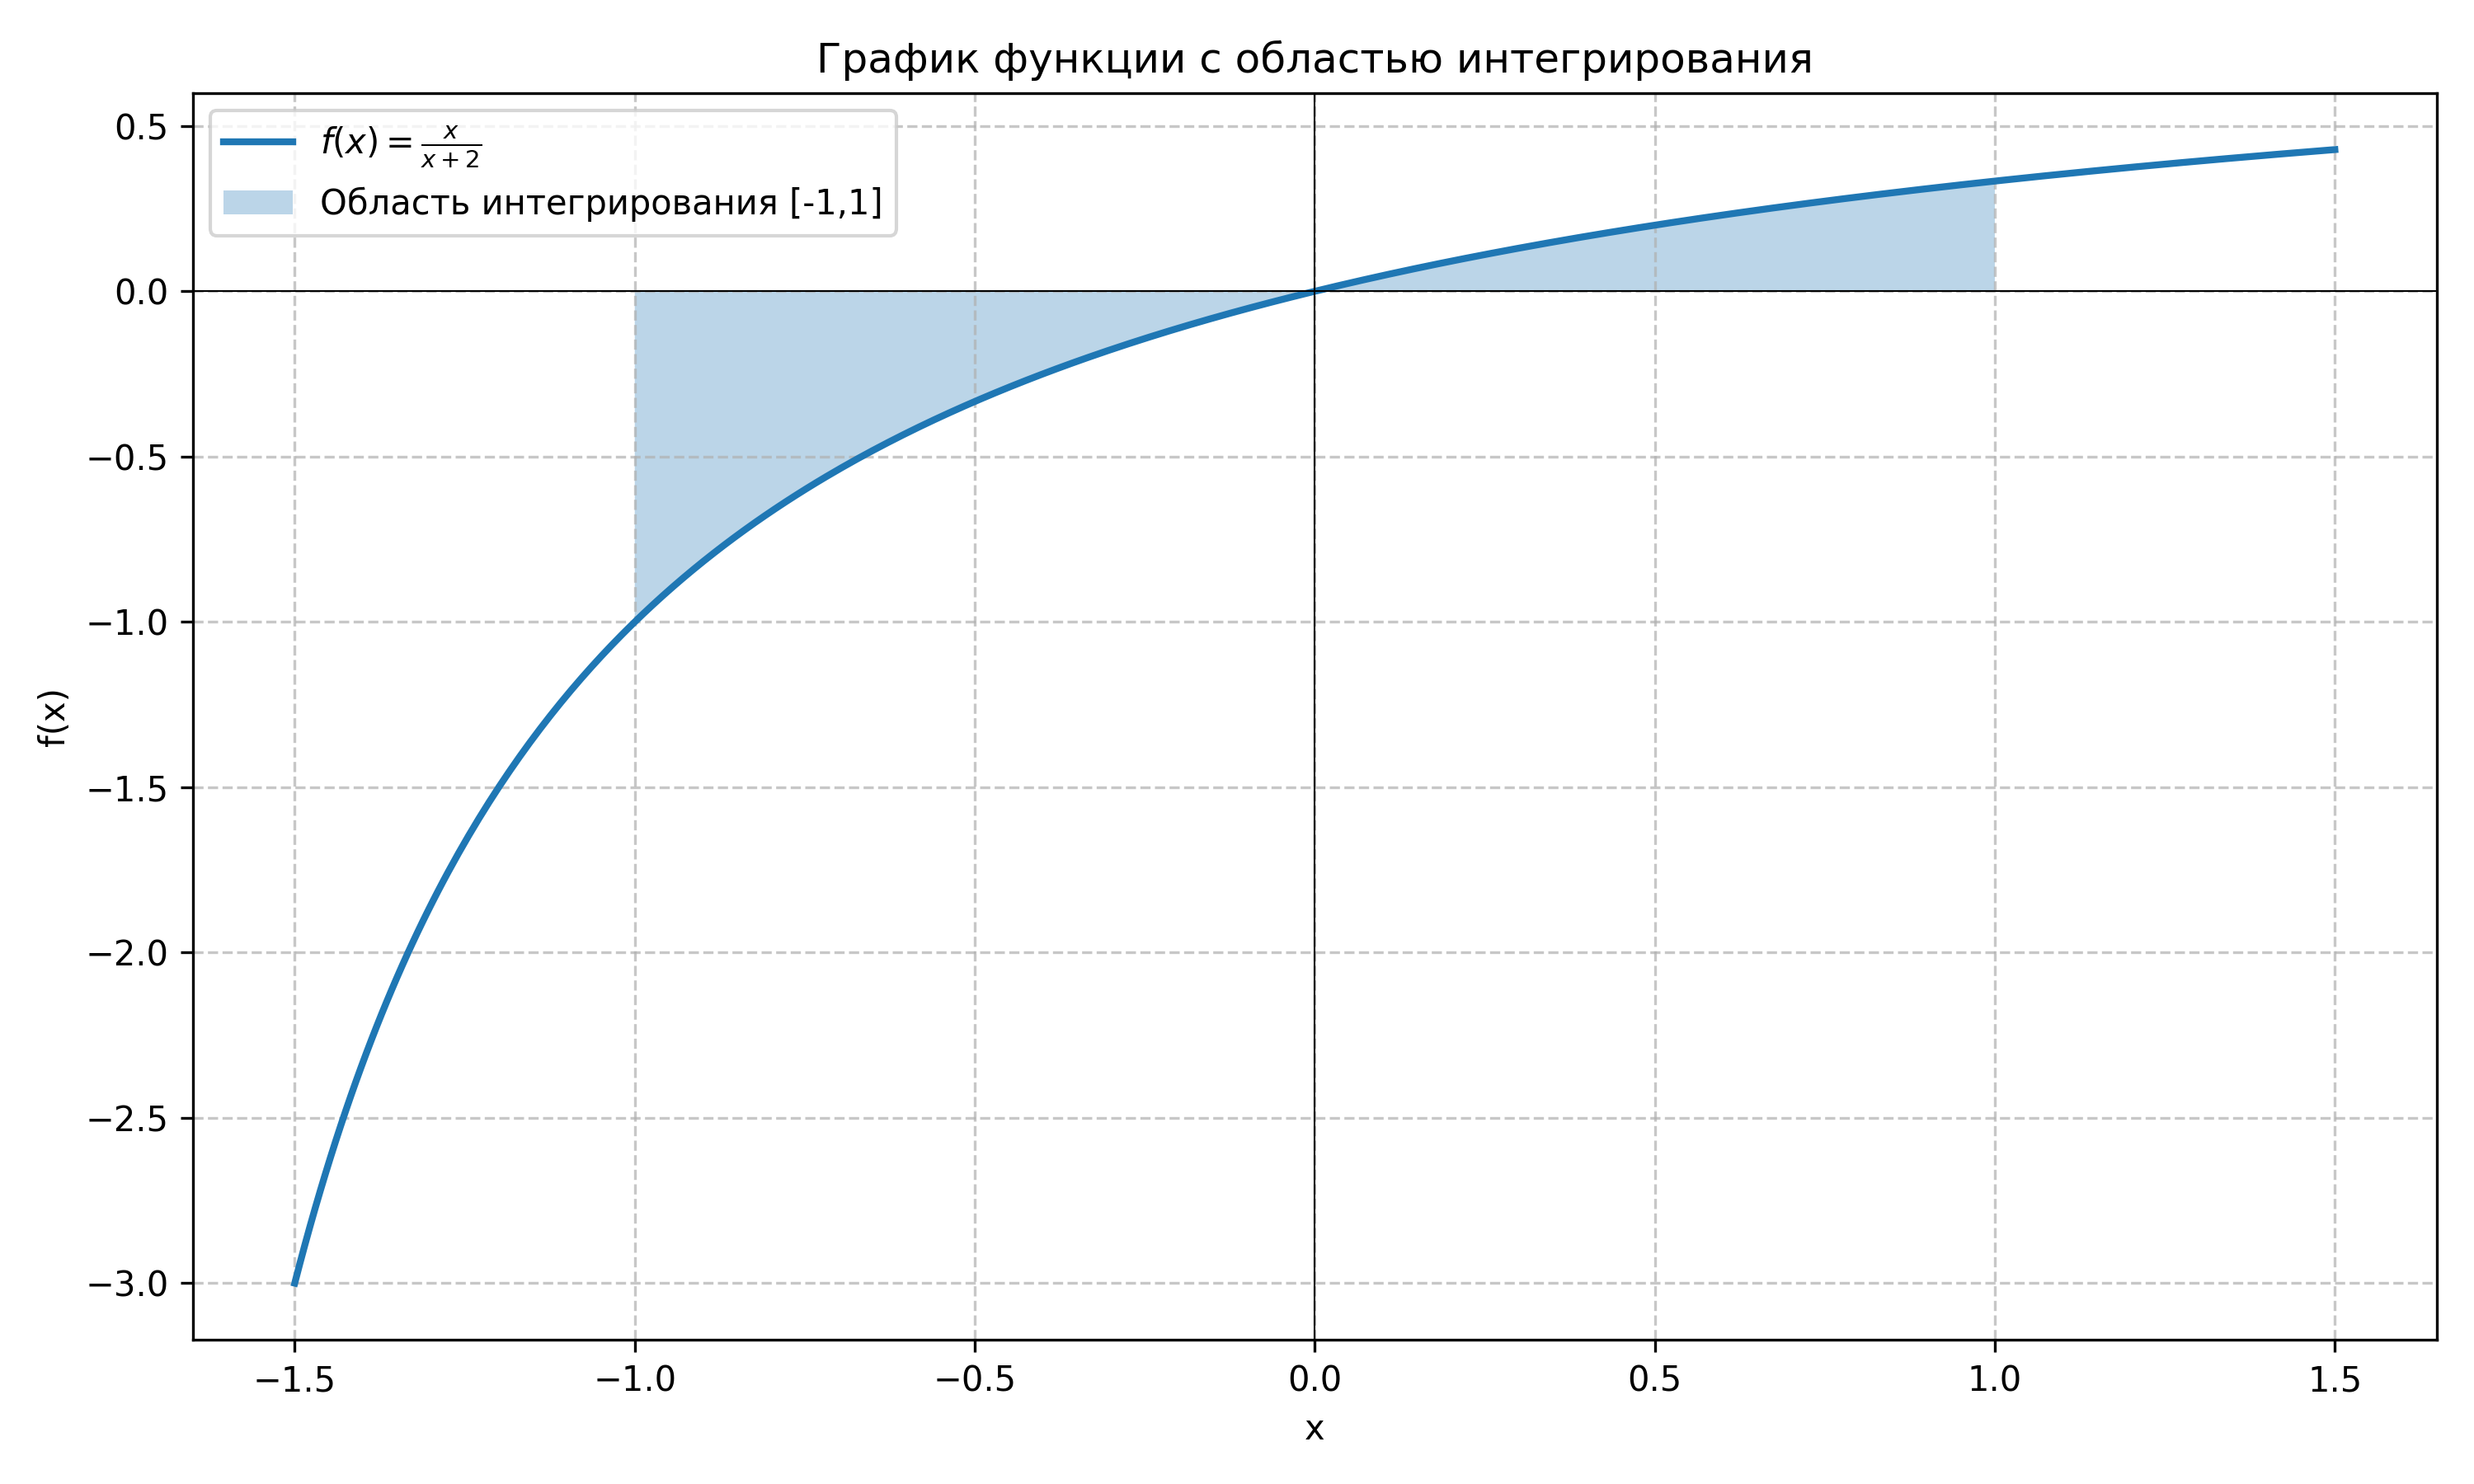
\includegraphics[width=0.9\linewidth]{img/integral_plot.png}
    \caption{График функции $f(x) = \frac{x}{x+2}$ с выделенной областью интегрирования $[-1,1]$}
    \label{fig:integral}
\end{figure}

\emph{Решение задачи:}

\begin{figure}[H]
    \centering
    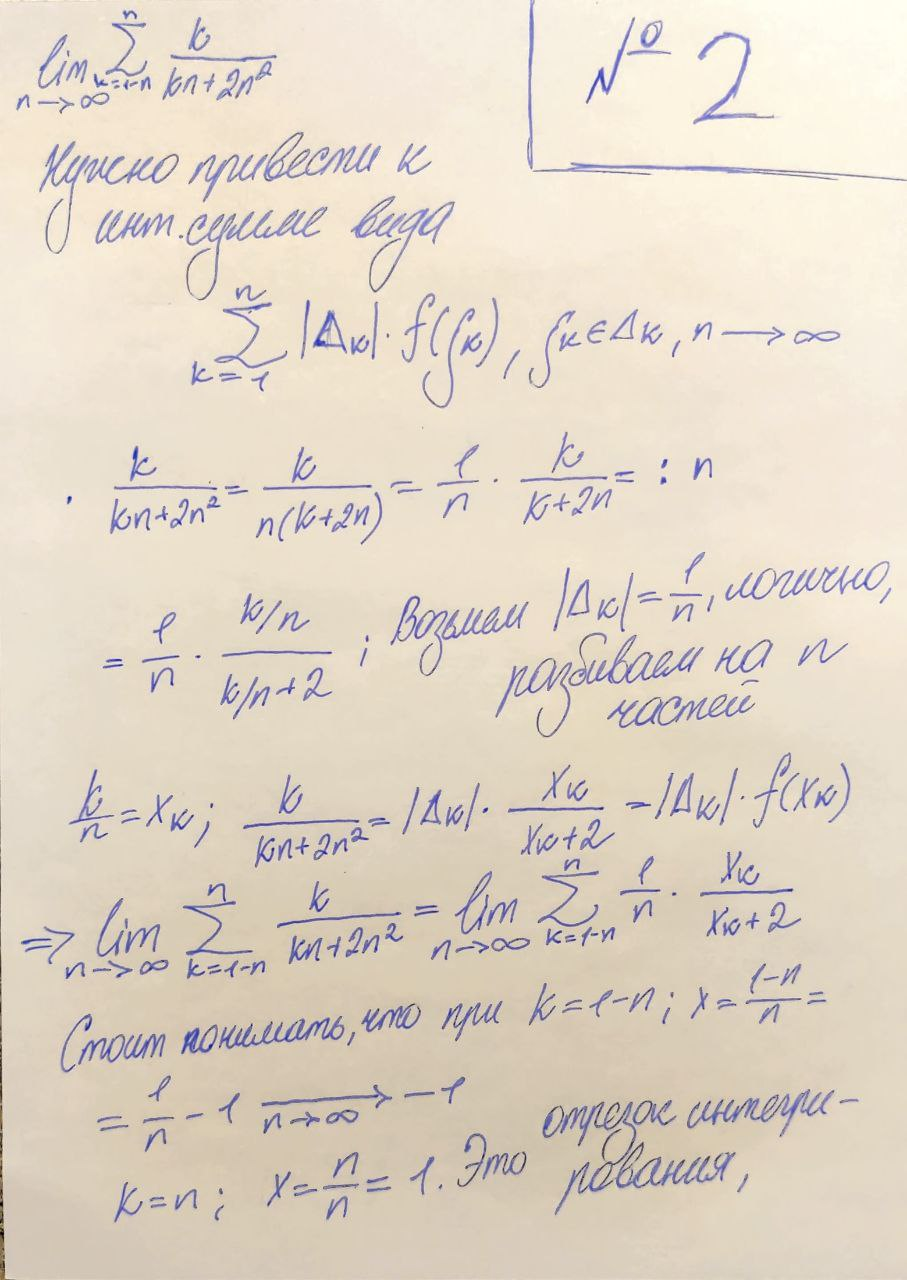
\includegraphics[width=0.8\linewidth]{img/2_1.jpg}
    \caption{}
    \label{fig:part1}
\end{figure}

\begin{figure}[H]
    \centering
    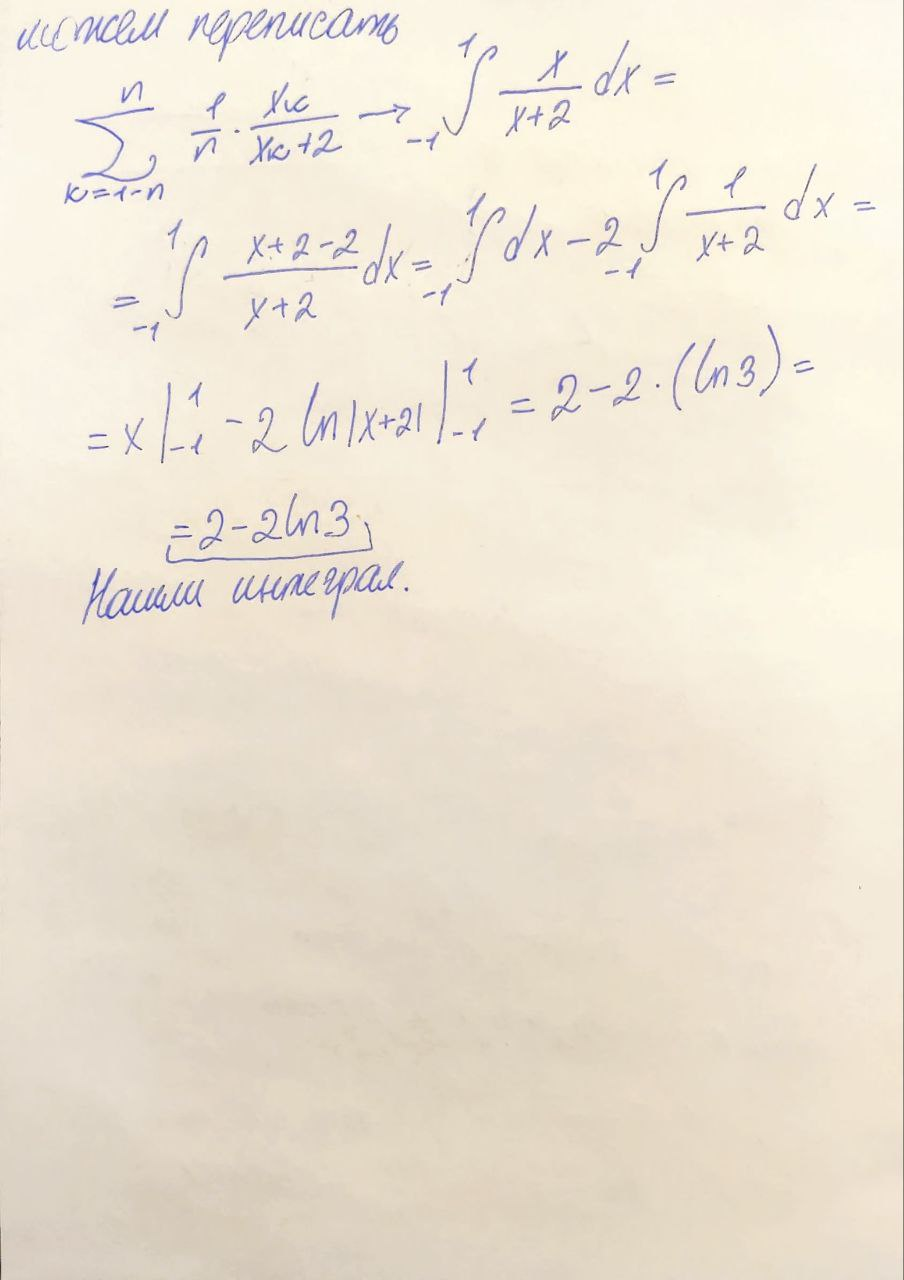
\includegraphics[width=0.8\linewidth]{img/2_2.jpg}
    \caption{}
    \label{fig:part2}
\end{figure}

Таким образом, легко выделилось количество промежутков интегрирования, сама функция от $x$, рассмотрел края и пришел к формуле Ньютона-Лейбница, вычислив определенный интеграл.\\
\emph{Задача решена}


\subsection{Задание 3}


\subsection{Задание 4}


\subsection{Задание 5}


\subsection{Задание 6}


\subsection{Задание 7}


\subsection{Задание 8}


\section{Выводы}

\end{document}

